\documentclass{article}

\usepackage{graphicx} % Required for the inclusion of images
\usepackage[utf8]{inputenc}
\usepackage{hyperref}

\title{AM4L: Applications Mobiles \\ Réalisation d'une application Android \\ ECAlendar \\
\vspace{1cm} \large{ECAM Bruxelles} \vspace{5cm}}

\author{Charles \textsc{Vandevoorde} (13019)\\
		Lorenzo \textsc{Riga} (13018)\\
		Antoine \textsc{Vander Meiren} (12088)\\
		Gaetano \textsc{Giordano} (12054)\\
		Sylvain \textsc{Alonso} (12150)\\}

\date{\vspace{5cm}\today}

\begin{document}

	\maketitle
    \newpage


	\section{Introduction}
    Dans le cadre du cours d'applications mobiles, nous avons réalisé une application Android
    "ECAlendar" à l'aide d'Android Studio. Cette dernière utilise l'API de "Ecam Calendar" afin de
    permettre aux étudiants de consulter leurs horaires directement sur leurs GSM.\\

    Dans ce rapport, nous allons présenter la manière dont nous nous sommes organisés en groupe mais
    aussi la structure de notre application ainsi qu'un listing de ses fonctionnalités.

	\section{Organisation du groupe}
	\hspace{0.45cm}
     Nous avons hébergé notre projet sur Github de manière à faciliter le travail en groupe et nous
     sommes répartis les tâches comme suit lors de la première séance:
	 \begin{description}
         \item[Charles] chargement des données depuis l'API, DAO ainsi que gestion de la
             \textit{RecyclerView}.
         \item[Lorenzo] gestion du layout, style de l'application.
         \item[Antoine] gestion des préférences, analyse est création des modèles requis et gestion de recherche de calendrier
         \item[Gaetano] gestion du layout et style de l'application.
         \item[Sylvain] intégration de la base de données SQLite et gestion des clics (affichage des détails lorsque l'utilisateur appuie sur un élément).
	 \end{description}


	\section{Présentation de l'architecture}
        \begin{figure}
            \centering
            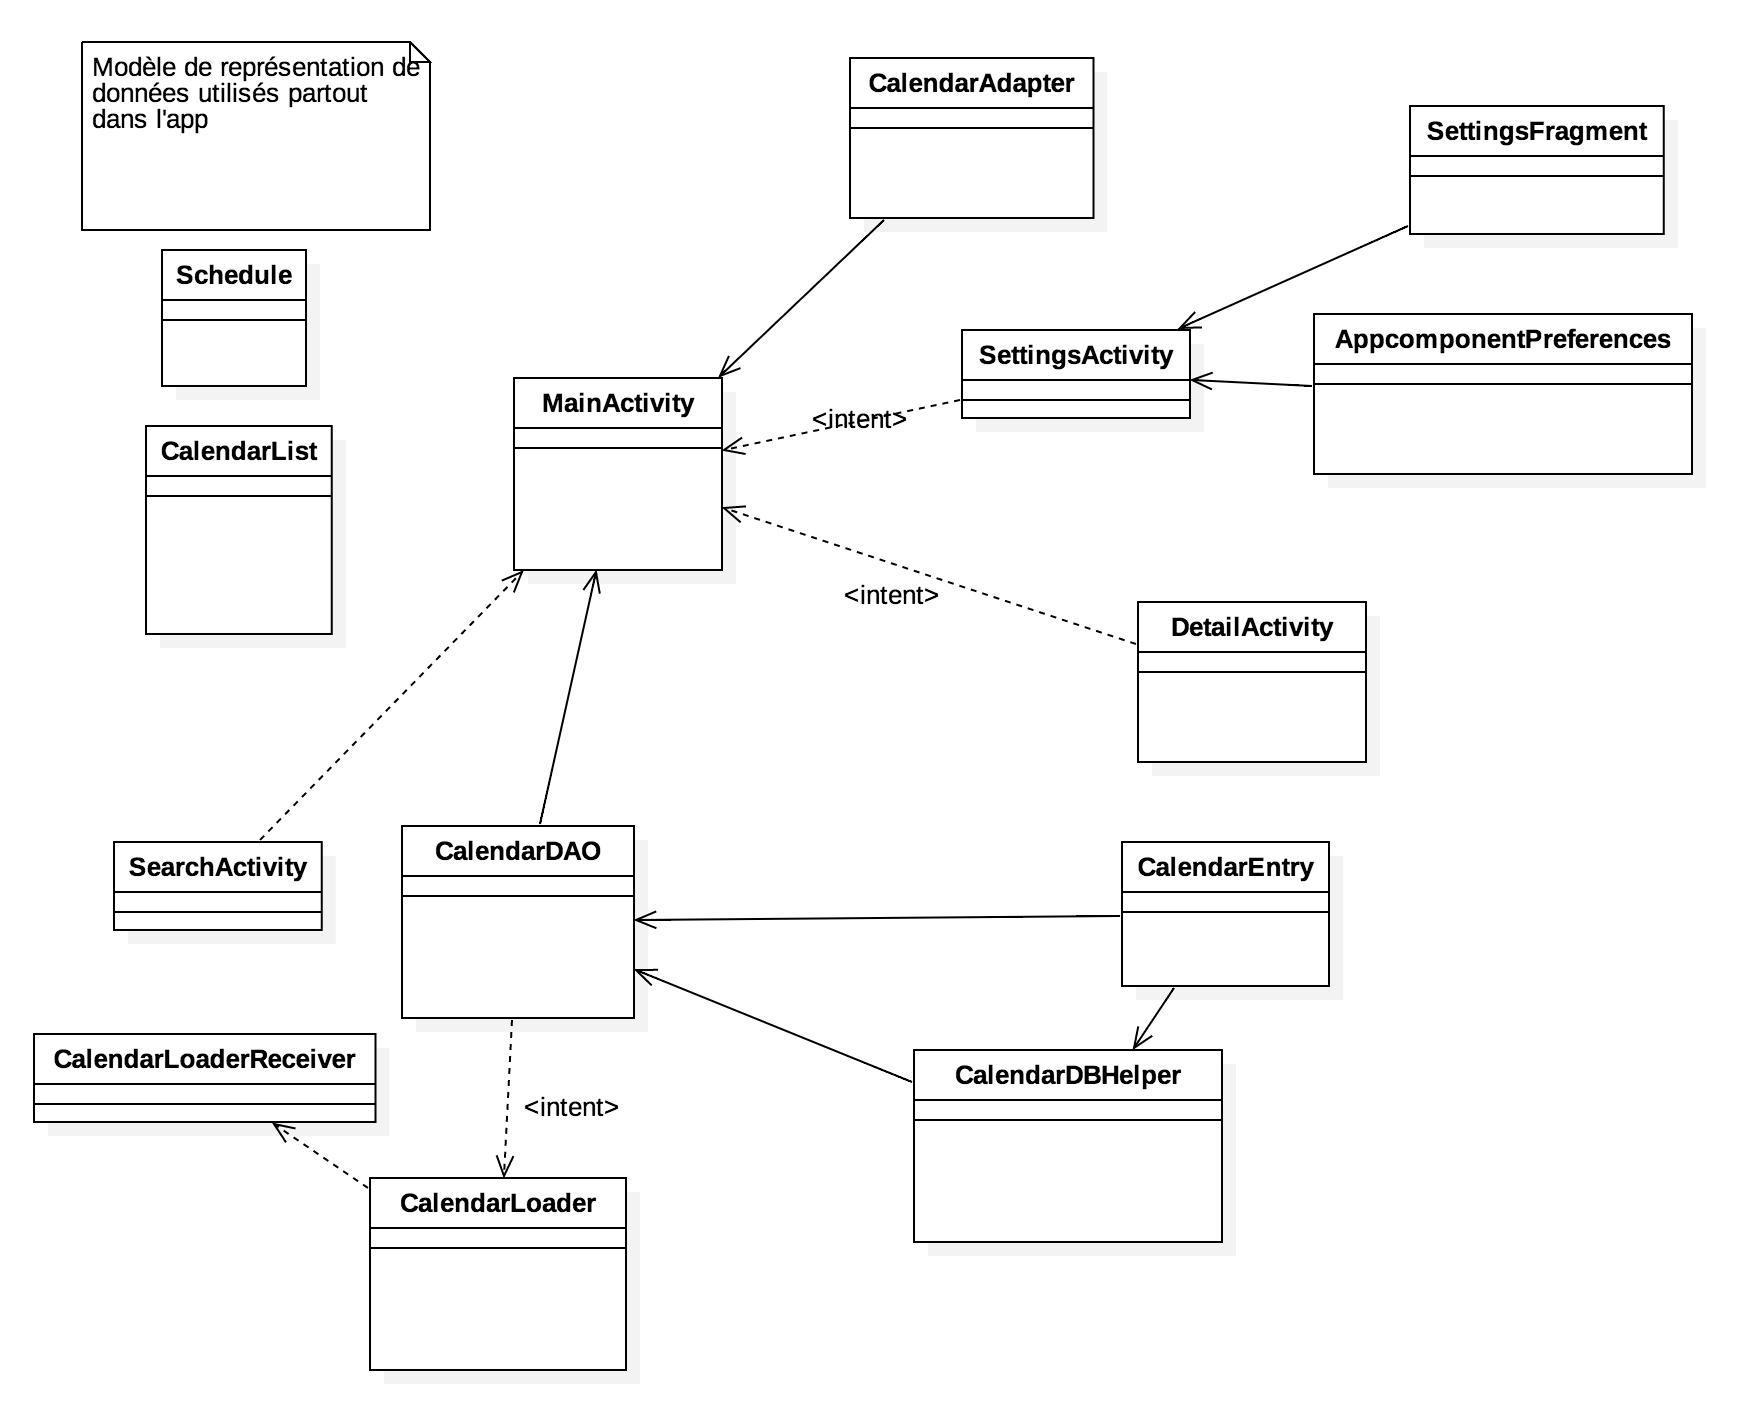
\includegraphics[scale=0.2]{img/uml.png}
            \label{fig:uml}
            \caption{Diagramme UML de classe représentant notre application}
        \end{figure}

	\subsection{Création des modèles}
		Avant de commencer à développer l'application, nous avons du analyser ce qui est renvoyé par
        l'API proposé par \textit{ECAM Calendar}
		afin de réaliser un modèle des données que nous allons devoir stocker. Nous avons décidé de créer deux modèles différents:
        \textit{Schedule} et \textit{CalendarType}. \
        \textit{Schedule} stocke toutes les informations relative à un calendrier en particulier: local, date et heure,
		professeur, note, nom de l'activité, personne concernée par groupe, \ldots \
        \textit{CalendarType} quant à lui permet de sauver les différents calendrier disponible via un ID et une description du l'année/section,
		du professeur ou du local. \

		Tout au long de l'application nous utiliserons ces modèles pour créer des objets utilisables par chacune des parties.

	\subsection{Gestion des préférences}
    Pour ce qui est des préférences, nous avons simplement effectué une \textit{PreferenceActivity}, accessible via le menu Android de l'application,
		et composée d'un fragment de préférence affichant une liste d'horaire disponible
		qui permet à l'étudiant de sélectionner son horaire personnel, en l'occurrence l'année dans laquelle il se trouve et sa série. \
		Au premier lancement de l'application, l'activité principale n'affichera pas de calendrier et nous demandera de nous rendre dans
		l'onglet préférence afin de sélectionner l'année désirée. \
		A partir de ce menu, nous avons développé une "Up Navigation" qui permet de retourner directement à la l'activité principale montrant
		le calendrier sélectionne. Notons que nous pouvons également utilisé le bouton back
        nativement présent sur les smartphones Android.

	\subsection{Recherche d'un second calendier}
		L'application permet à l'utilisateur de sélectionner deux calendrier à la fois: le sien
        comme principale via les préférences et
		un second pour pouvoir comparer deux calendrier par exemple.  \
        Pour en sélectionner un second, nous avons ajouté une petite loupe dans le menu Android de l'application qui nous amène à une autre
        activité nommée \textit{SearchActivity}. Cette activité nous montre une liste, scrollable,
        de tous les calendriers disponible via l'API calendrier de l'ECAM.
		En cliquant une seconde fois sur cette loupe nous faisons apparaitre un clavier qui permet de rentrer du texte afin de rechercher
		un calendrier particulier. \
		La recherche permettra à l'utilisateur de visualiser au fur et à mesure qu'il tape, les calendriers disponible en fonction du
		texte qu'il complète afin de simplifier la sélection désirée. \\
		L'utilisateur pourra ensuite cliquer  sur le calendrier de son choix, il recevra une
        confirmation de ce choix via un message \textit{Toast},
		et pourra retourner à l'activité principale via la "Up Navigation" ou encore le bouton back natif android. La valeur du calendrier
        sera alors stockée dans un \textit{SharedPreference} disponible pour le reste de l'application.
		Une fois sur l'activité principale, le second calendrier sera disponible pour l'utilisateur. \
		A chaque redémarrage de l'application ou changement de la section dans les préférences de
        l'application (\textit{onDestroy} de la \textit{MainActivity}),
        cette \textit{SharedPreference} sera remise à zéro pour ne plus apparaitre dans le calendrier principale de l'utilisateur.


        \subsection{Récupération des données depuis l'API REST}
            Notre application pour fonctionner a besoin de données provenant de l'API REST du site
            \url{calendar.ecam.be}. Après une analyse des requêtes faites par l'application web
            Calendar, nous avions tous les outils en main pour démarrer l'implémentation de l'API
            dans notre application.

            Pour éviter de bloquer l'interface utilisateur pendant le chargement des données, nous
            avons utilisé un \textit{IntentService}. Celui-ci est un service spécial d'Android qui
            s'arrête dès que la tâche est finie. Nous avons choisi ce type de service à la place de
            système comme les \textit{AsyncTaskLoader}, \ldots pour plusieurs raisons.
            \begin{itemize}
                \item Meilleur séparation des affaires puisqu'un \textit{IntentService} ne doit pas
                    obligatoirement être appelé de l'activité principale.
                \item API plus propre grâce à l'utilisatation d'\textit{Intent}.
            \end{itemize}

            Notre service peut être appelé pour récuperer deux types de données: la liste des
            calendriers disponibles (profs, locals, séries, \ldots) et un calendrier. Pour chaque
            type, nous envoyons la requête via un \textit{Intent} contenant les données nécessaires
            à la récupération des données.

            Les requêtes HTTP sont faites synchrone à l'aide de \textit{future} puisqu'Android ne
            supporte pas le multi-threading imbriqué. Pour ce faire, nous avons utilisé la librairie
            \textit{Volley} qui est une nouvelle libraire permettant de faciliter les requêtes HTTP.

            L'utilisation des \textit{futures} vient du fait que \textit{Volley} est asynchrone de
            base.

            Le parsing des données ICS (format de donnée de calendrier) est effectué par une
            libraire appelée \textit{iCal4j}. Le parsing est effectué dans l'\textit{IntentService}
            pour éviter des ralentissements inutiles de l'interface utilisateur.

            Finalement, les données sont renvoyés via un \textit{Broadcast} jusqu'à un récepteur
            spécialement écrit pour ce service. Nous détaillerons plus en détail ce récepteur dans
            la section \ref{sec:dao}.

        \label{sec:dao}
        \subsection{Le DAO}
            DAO signifie \textit{Data Access Object}. Cette classe permet d'être le seul point
            d'accès aux données et décide de quel source les données seront tirées. Dans notre cas,
            les sources sont la base de donnée et l'API REST du site \url{calendar.ecam.be}.

            La sélection de la source est assez trivial, nous regardons d'abord si les données sont
            en base de données et si elles sont assez nouvelles (moins de 1 semaines) aussi non,
            nous allons utilisés notre \textit{IntentService} pour charger nos données et les sauver
            dans la base de donnée.

            Mise à part la création, le DAO est responsable de la sauvegarde et de la reprise de
            données en base de données.

            Le DAO devant gérer l'asynchronisme de l'\textit{IntentService}, nous avons utilisés un
            système de "notifieurs" qui demande d'être notifié dès qu'une donnée est arrivée. Le DAO
            garde donc une liste de classe implémentant une certaine interface.

            Une autre caractéristique du DAO est que celui-ci est implémenté comme un singleton
            parce que nous devions avoir le contexte d'une activité pour sauvegardé les données en
            base de données. Lorsque le \textit{CalendarLoaderReceiver} (le récepteur de
            l'\textit{IntentService}) reçoit les données, nous devons accéder au DAO mais le
            récepteur n'a pas de contexte. Il faut donc avoir un contexte statique (mauvaise pratique
            en général) ou alors implémenter le DAO entant que singleton. Cette décision nous a
            permis également d'être beaucoup plus flexible quand au chargement des données.

        \subsection{Le \textit{RecyclerView}}
            Le \textit{RecyclerView} nous permet d'afficher une grande liste de calendriers sans
            problème de performances. Dans notre cas, nous avons créer une \textit{RecyclerView}
            avec deux types de données. Nous pouvions soit avoir un slot horaire, soit avoir une
            information sur la date des slots horaires suivant.

            Dans notre \textit{ItemAdapter} qui gère la création à la volée des informations
            affichées, nous avons donc deux différents \textit{ViewHolder}.

            La \textit{RecyclerView} ne supportant qu'une seule liste de donnée, nous avons créer
            une liste d'\textit{Object}. Cette approche pourrait être changé dans le futur si nous
            rajoutons plusieurs types de vues différentes. Dans notre cas, cette solution est la
            plus facile et la plus rapide à implémenter.

	\section{Listing des fonctionnalités}
    \begin{itemize}
        \item Affichage de calendrier reprenant son horaire personnel
        \item Recherche parmi les calendrier disponible via l'API de l'ECAM
        \item Affichage simultané d'un second calendrier au choix pour comparer des horaires (local, professeur et étudiant)
    \end{itemize}

	\subsection{Icône}
	 Que serait une application mobile, sans une icône appropri\'ee. C'est pour cela que nous avons cr\'ee une icône ECAlendar spécialement customis\'ee pour notre application.
	   \begin{center}
            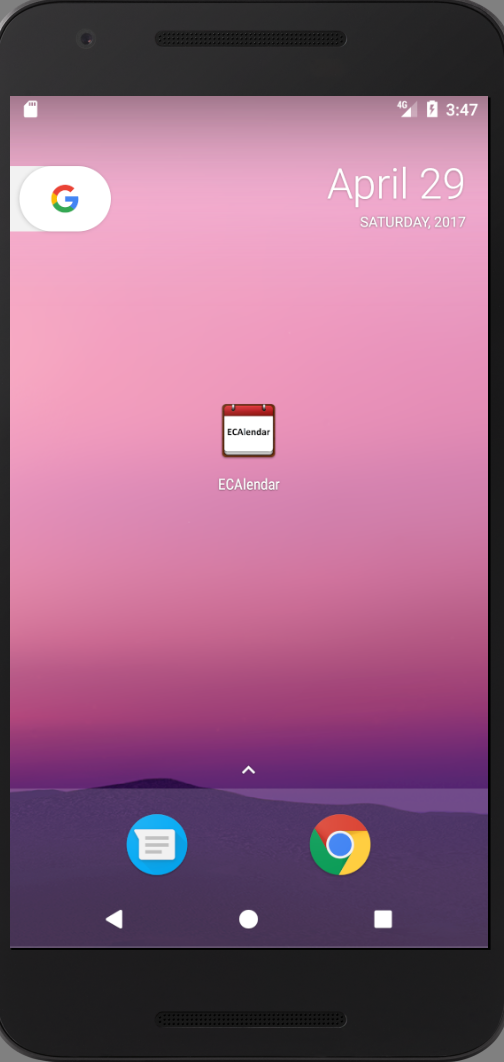
\includegraphics[scale=0.4]{img/ICON.png}
        \end{center}



	 \subsection{La page d'accueil}
	 Comme vous pouvez le voir sur l'image, en entrant dans l'application ECAlendar nous avons une page qui nous indique les cours pour l'ann\'ee s\'electionn\'ee. Autrement dit elle indique la date ainsi que les cours donn\'es. Elle indique \'egalement l'heure du début et l'heure de fin du cours.
	   \begin{center}
            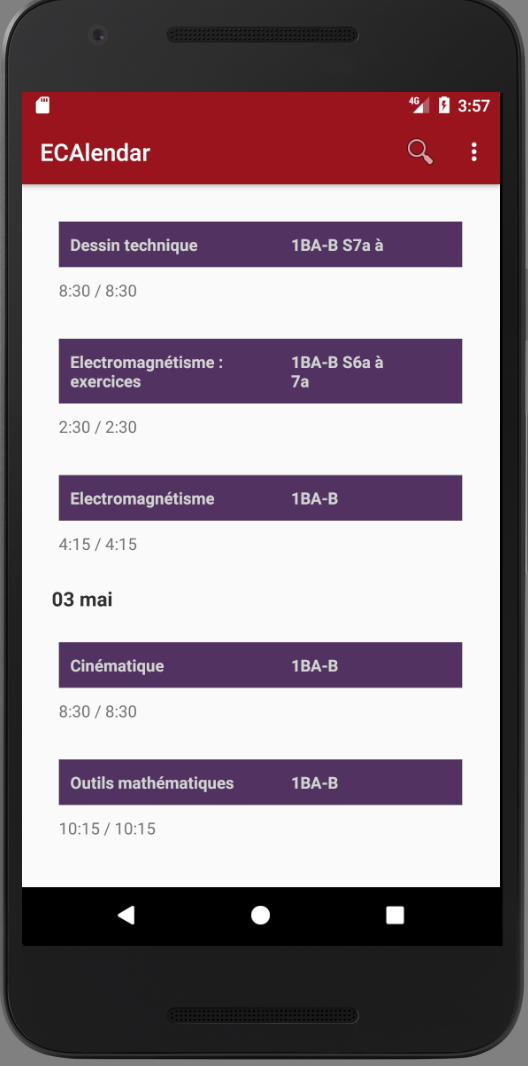
\includegraphics[scale=0.4]{img/Page_Accueil.png}
        \end{center}


	 \subsection{D\'etail d'un cours}
	 En cliquant sur l'un des cours on entre dans une nouvelle page qui nous permet d'afficher les d\'etails concernant ce cours. C'est a dire le local, l'enseignant et la s\'erie.
        \begin{center}
            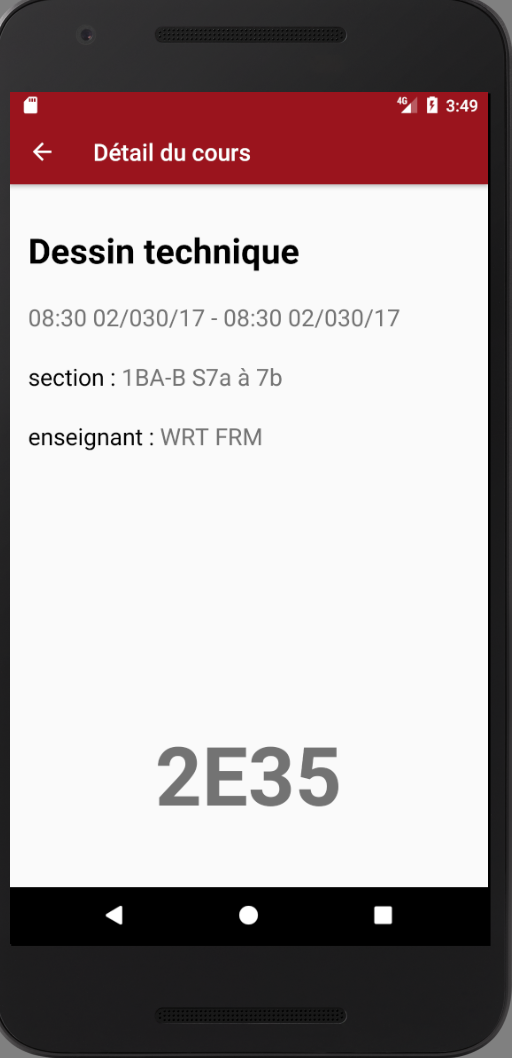
\includegraphics[scale=0.4]{img/Section.png}
        \end{center}

            \subsection{Choix de l'ann\'ee}
	Bien évidement, notre application nous permet de choisir \'egalement l'ann\'ee d'\'etude pour lequel nous aimerions voir l'horaire. C 'est pour cela que sur la page d'accueil en  cliquant sur les 3 points  en haute \`a droite, cela nous redirigera vers une page qui nous permettra de cocher une ann\'ee et ainsi la mettre dans nos pr\'eferences.
        \begin{center}
            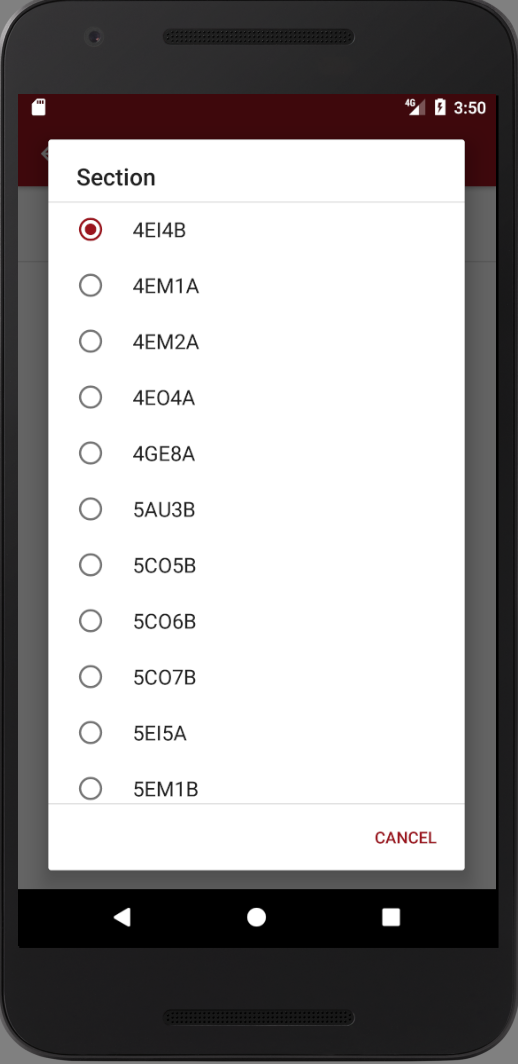
\includegraphics[scale=0.4]{img/Annee.png}
        \end{center}

	\subsection{Recherche}
	Nous pouvons \'egalement choisir l'ann\'ee sur la page d'accueil, en cliquant simplement sur la petite loupe situ\'ee en haut. Cela nous redirigera vers la page ci-dessous.
        \begin{center}
            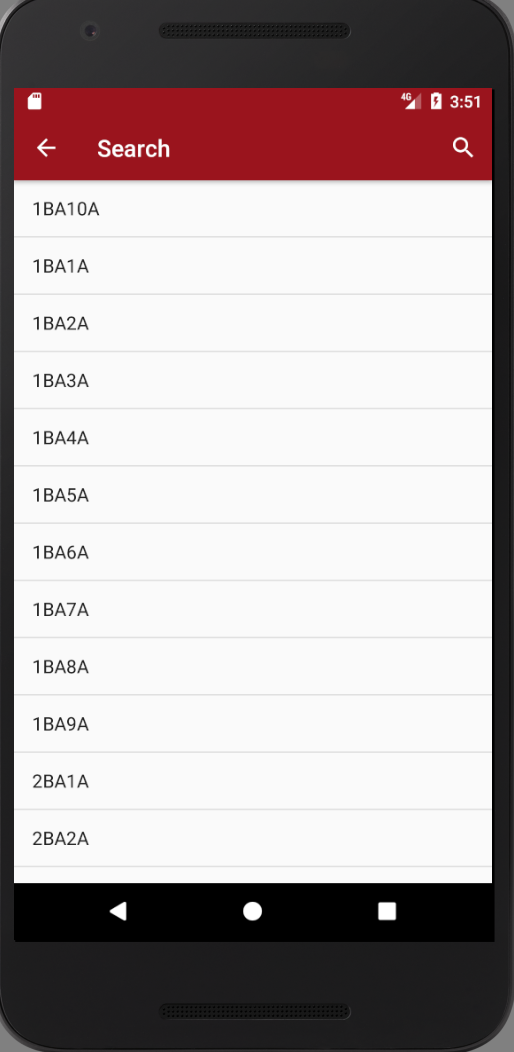
\includegraphics[scale=0.4]{img/search.png}
        \end{center}

          \subsection{Remarques}
          Comme vous pouvez le voir sur certaines images, certains bugs interviennent comme par exemple l'heure de fin du cours. Nous tenons a pr\'eciser que ces bugs ont \'et\'e corrig\'es et fonctionnent d\'esormais parfaitement.

    \section{Conclusion}
	La réalisation de cette application nous aura permis de nous familiariser avec les notions vues lors des différents cours théoriques ainsi que d'améliorer notre organisation en groupe dans le cadre d'un projet de développement. \\
	
	Nous avons atteint les objectifs que nous nous étions fixés en réalisant une application fonctionnelle et user-friendly reprenant l'ensemble des fonctionnalités auxquelles nous avions pensé lors de la première séance.
\end{document}
